\documentclass[12pt]{article}

\usepackage{amssymb, amsmath, amsfonts}
\usepackage{amsthm}
\usepackage{moreverb}
\usepackage{graphicx}
\usepackage{enumerate}
\usepackage{graphics}
\usepackage{listings}
\usepackage{color}
\usepackage{array}
\usepackage{float}
\usepackage{hyperref}
\usepackage{textcomp}
\usepackage{caption}
\usepackage{alltt}
\usepackage{mathtools}
\usepackage[T1]{fontenc}
\usepackage{fullpage}
\usepackage{tikz}
\usepackage[utf8]{inputenc}
\newcommand{\suchthat}{\, \mid \,}
\usepackage{fancyvrb}
%\allowdisplaybreaks
\def\arraystretch{1.7}%  1 is the default, change whatever you need

\definecolor{codegreen}{rgb}{0,0.6,0}
\definecolor{codegray}{rgb}{0.5,0.5,0.5}
\definecolor{codepurple}{rgb}{0.58,0,0.82}
\definecolor{backcolour}{rgb}{0.95,0.95,0.92}
 
\lstdefinestyle{mystyle}{
    backgroundcolor=\color{backcolour},   
    commentstyle=\color{codegreen},
    identifierstyle=\color{blue},
    keywordstyle=\color{magenta},
    numberstyle=\tiny\color{codegray},
    stringstyle=\color{codepurple},
    basicstyle=\footnotesize\ttfamily,
    breakatwhitespace=false,         
    breaklines=true,                 
    captionpos=b,                    
    keepspaces=true,                 
    numbers=left,                    
    numbersep=5pt,                  
    showspaces=false,                
    showstringspaces=false,
    showtabs=false,                  
    tabsize=2
}
 
\lstset{style=mystyle}

\begin{document}

{\bf MATH 481A \hfill Numerical Analysis \ \ \ \ \ \hfill Spring 2015}

\title{\bf Lab \# 3 Solutions}
\author{\bf Sam Fleischer}
\date{\bf Tues. Mar. 24, 2015}

{\let\newpage\relax\maketitle}
\maketitle
\tableofcontents
\pagebreak

\section*{Problem 1}
\addcontentsline{toc}{section}{Problem 1}
{\it Write a Python function that takes as input the integer {\tt n} are returns a 1d {\tt numpy} array of lenth {\tt n} holding the {\tt n} roots of unity; that is, the {\tt n} roots of the polynomial $z^n - 1 = 0$.}

\begin{lstlisting}[language=Python, caption=Roots of Unity FUnction] 
def roots_of_unity(n):
    zeros = np.zeros(n, complex)
    for i in xrange(0, n):
        zero = math.cos((2*math.pi/n)*i) + math.sin((2*math.pi/n)*i)*1j
        zeros[i] = zero

    return zeros
\end{lstlisting}

\section*{Problem 2}
\addcontentsline{toc}{section}{Problem 2}
{\it Write a Python function named {\tt nfractal} that takes as input four arguments: {\tt K}, {\tt pixel}, {\tt tol}, and {\tt n}, and}
\begin{enumerate}[\it\ \ 1.\ \ ]
    \item {\it generates a mesh of the complex plane consisting of {\tt pixel} points along the $x$-axis and {\tt0.75*pixel} points along the $y$-axis, with $x,y\in [-1.5, 1.5]$.}
    \item {\it applies the iteration $z_{k+1} = z_k - a\left(\dfrac{p(z_k)}{p'(z_k)}\right)$ to each $z = x + iy$ on the mesh {\tt K} times and records the number of times that the iterated value is within {\tt tol} distance to one of the roots of the polynomial $p(z)$.}
    \item {\it colors each point in the mesh grid according to the number of times it is within a distance {\tt tol} of one of the roots of the polynomial $p(z)$.}
\end{enumerate}

\begin{lstlisting}[language=Python, caption=Newton Fractal Function] 
def nfractal(K, pixel, tol, n):
#generates the newton fractal for a given polynomial

    r = 0.75
    a = alpha + beta*1j

    limit = 1.5

    x = np.linspace(-limit, limit, pixel)
    y = np.linspace(-limit, limit ,round(pixel*r))

    [Re, Im] = np.meshgrid(x,y)
    C = np.zeros([round(r*pixel), pixel], complex)
    C = Re + Im*1.0j

    B = np.zeros([round(r*pixel), pixel], float)
    Id = np.ones(B.shape)

    zeros = roots_of_unity(n)
    iteration = define_iterative_method(n, a, Id, zeros, tol)
    
    Cn = C
    
    for k in range(1,K):
        (Cn, B) = iteration(Cn, B)
        if k % 10 == 0:
            print k

    plt.pcolormesh(x, y, B, cmap = color) # bone, copper, summer
    file_name = "fractal_%d_%d_%d.png" % (K, pixel, n)
    plt.savefig(file_name, format="png", dpi = 150)
    print file_name
\end{lstlisting}
Line 20 defines the iterative method for line 25 by calling the following function:
\begin{lstlisting}[language=Python, caption=Definition of the Iterative Method]
def define_iterative_method(n, a, Id, zeros, tol):
    def iteration(Cn, B):
        Cn -= a*(Cn**n - Id) / (n*Cn**(n-1))
        for i in xrange(0, n):
            B += (i)*(np.abs(Cn - Id*zeros[i]) < tol)
        return (Cn, B)
    return iteration
\end{lstlisting}

\noindent {\it Apply the iteration for polynomials of the form $p(z) = z^n - 1$ for values of $n = 2,3,4$, and different $complex$ values of $a$.  This will generate the {\underline{Julia Set}} of the rational function $z_{k+1} = z_k - a\left(\dfrac{p(z_k)}{p'(z_k)}\right)$ for the polynomial $p(z)$.  Repeat the calculation for different values of {\tt pixel}, {\tt K}, and {\tt tol}, and try different {\tt matpoltlib} color maps until you obtain a fractal you like.}\\

\noindent {\it Repeat the images you created above but coloring the points on the grid according to the root they converge to. That is, if the $k$\textsuperscript{th} iteration of the point $z_{m,n} = x_m + iy_n$ is closest to the $s$\textsuperscript{th} root, increase the counter of that point and not the others and making sure that points that converge to one root end up being colored differently than those converging to another root.} \\

\noindent The following images were created from various runs of the code.  The number of iterations, the number of pixels, the tolerance, the number of complex roots in the polynomial $z^n - 1$, the value of $a$, and the color scheme were all parameters passed through the command line.  For the last four images, the range was changed to $x, y \in [-2, 2]$.

\begin{figure}[H]
    \centerline{
        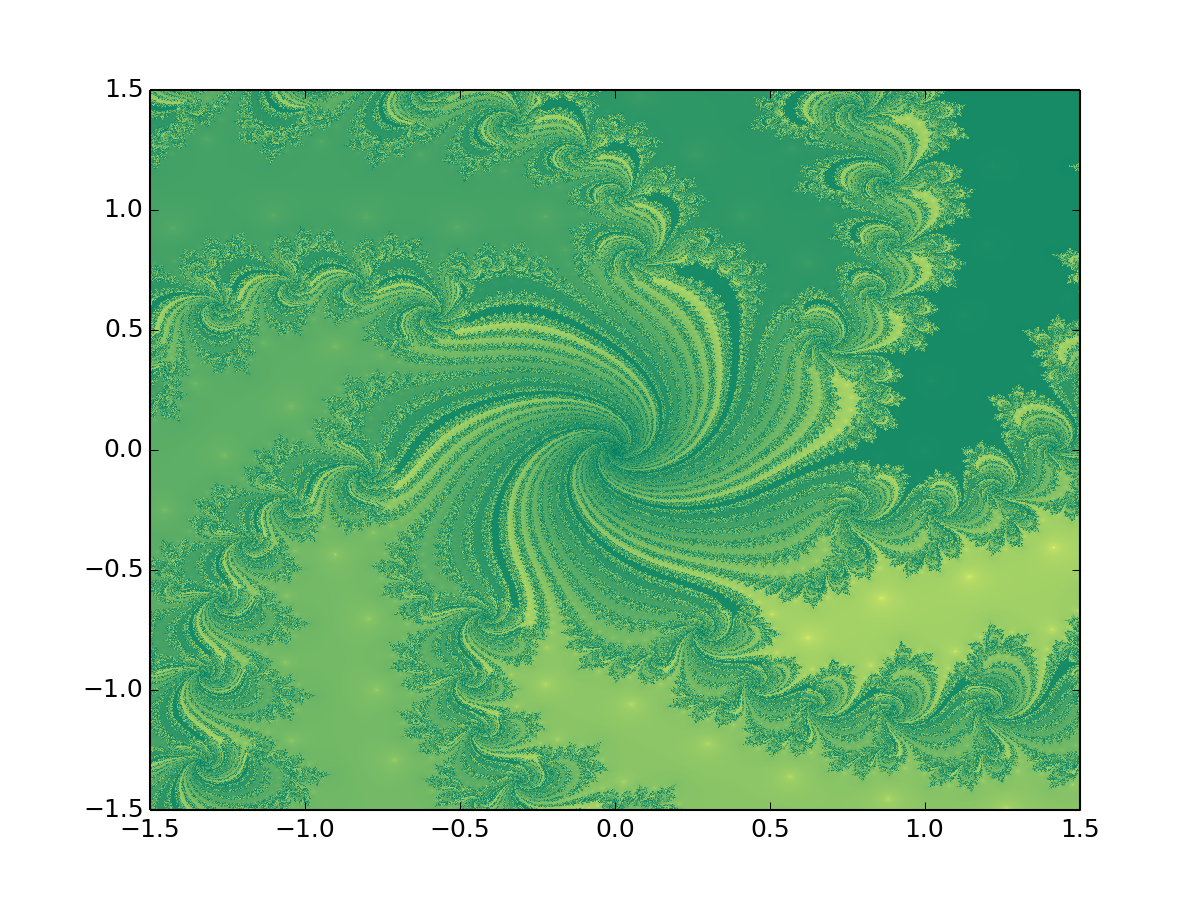
\includegraphics[scale=1.1]{fractal_500_2500_7.png}
    }
    \caption*{$z^7 - 1 = 0$, $a = 1 + \frac{19}{20}i$}
\end{figure}
\begin{figure}[H]
    \centerline{
        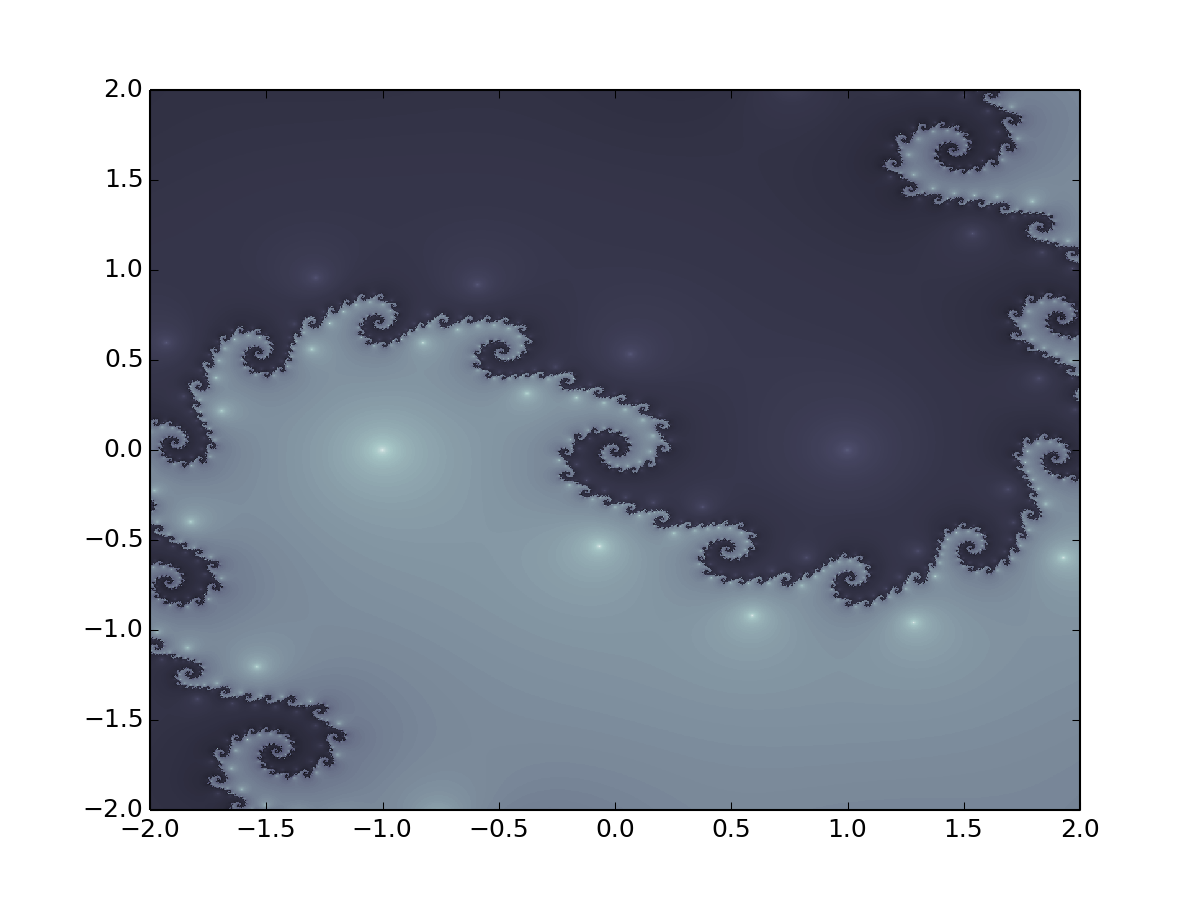
\includegraphics[scale=0.63]{fractal_250_1500_2.png}
    }
    \caption*{$z^2 - 1 = 0$, $a = \frac{1}{2} + \frac{3}{4}i$}
\end{figure}
\begin{figure}[H]
    \centerline{
        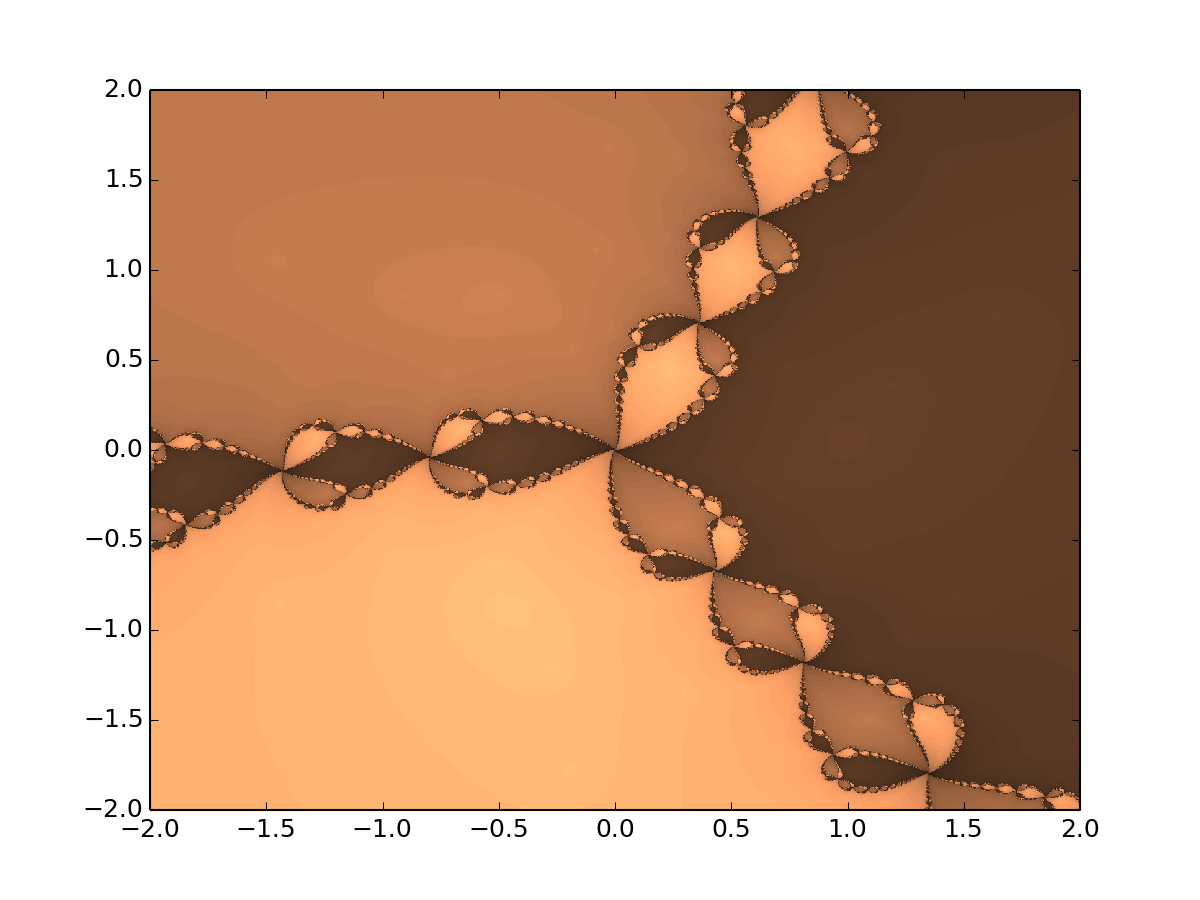
\includegraphics[scale=0.63]{fractal_50_1500_3.png}
    }
    \caption*{$z^3 - 1 = 0$, $a = 1 + \frac{1}{20}i$}
\end{figure}
\begin{figure}[H]
    \centerline{
        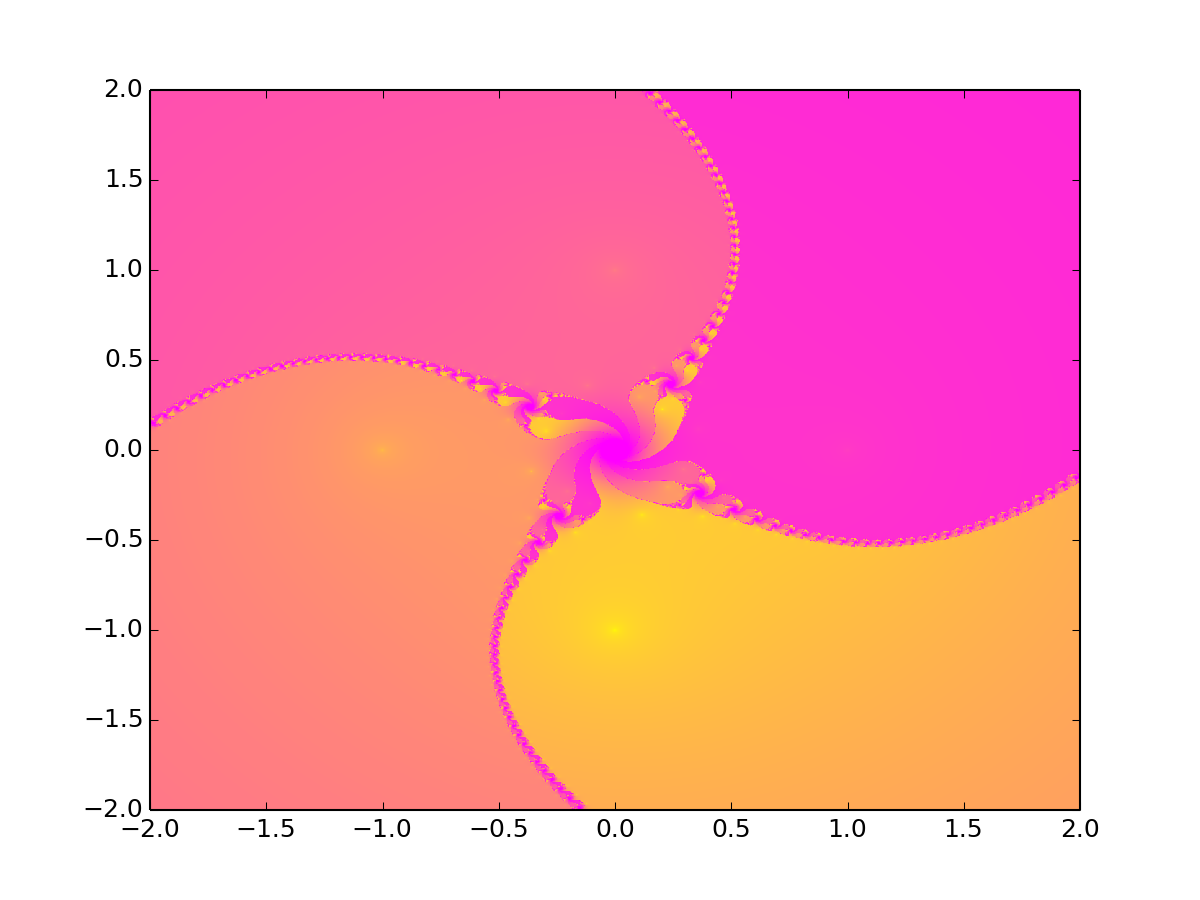
\includegraphics[scale=0.63]{fractal_350_1500_4.png}
    }
    \caption*{$z^4 - 1 = 0$, $a = \frac{1}{10} + \frac{1}{10}i$}
\end{figure}
\begin{figure}[H]
    \centerline{
        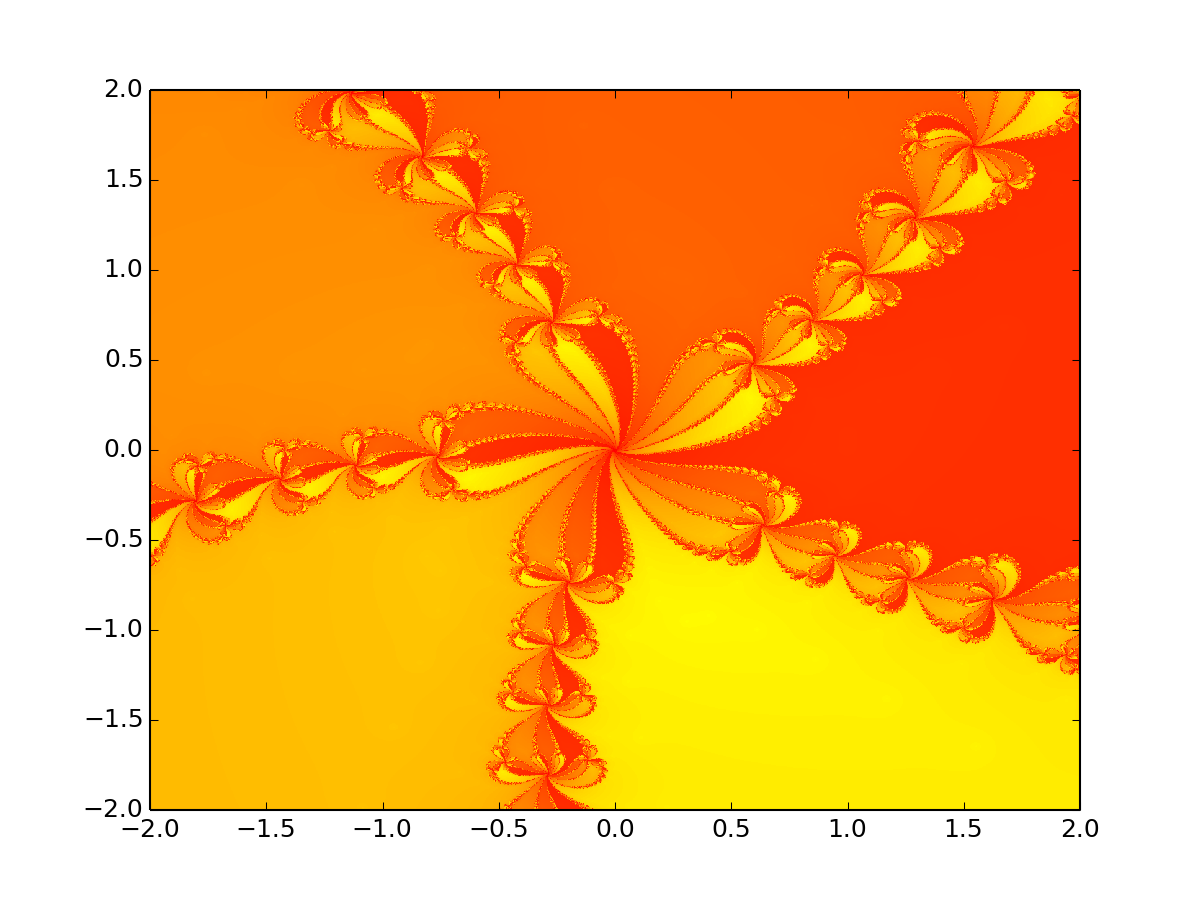
\includegraphics[scale=0.63]{fractal_100_1500_5.png}
    }
    \caption*{$z^5 - 1 = 0$, $a = 1 + \frac{1}{5}i$}
\end{figure}

%\pagebreak
%\begin{thebibliography}{99}
%
%\bibitem{Abrams1997b}
%Abrams, P.~A. and Matsuda, H.
%Prey Adaptation as a Cause of Predator-Prey Cycles.
%\emph{Evolution}
%1997, 51:1742-1750.
%
%\bibitem{Chavez2001}
%Brauer, F., Castillo-Chavez, C.
%Mathematical Models in Population Biology and Epidemiology.
%Springer,
%2011. Print.
%
%\bibitem{Boyce2012}
%Boyce, W. E., and DiPrima, R. C.
%Elementary Differential Equations and Boundary Value Problems %10\textsuperscript{th} ed.
%Wiley Global Education
%2012. Print.
%
%\bibitem{Saloniemi1993}
%Saloniemi, I.
%A Coevolutionary Predator-Prey Model with Quantitative Characters.
%\emph{American Naturalist}
%1993, 141:880-896.
%
%\bibitem{Schreiber2011}
%Schreiber, S.~J., B$\ddot{\mbox{u}}$rger,  R., and Bolnick,  D.~I.
%The Community Effects of Phenotypic and Genetic Variation within a Predator %Population.
%\emph{Ecology}
%2011,  92(8):526-543. 
%
%\end{thebibliography}

\end{document}